\documentclass{beamer}

\usepackage{cmap}
\usepackage[T1,T2A]{fontenc}
\usepackage[utf8]{inputenc}
\usepackage[russian]{babel}

\mode<presentation> {
\usetheme{Madrid}
\setbeamertemplate{caption}[numbered]
}

\usepackage{graphicx} % Allows including images
\usepackage{booktabs} % Allows the use of \toprule, \midrule and \bottomrule in tables

\title[Системное программирование]{MSDN: системные сервисы (часть 1)}

\author{Мартынов Семён}
\institute[СПб ПУ]
{
Санкт-Петербургский государственный политехнический университет \\
\medskip
\textit{semen.martynov@gmail.com}
}
\date{\today}

\begin{document}

\begin{frame}
\titlepage
\end{frame}

\begin{frame}
\frametitle{Содержание}
\tableofcontents
\end{frame}

%------------------------------------------------
\section{Введение}
%------------------------------------------------

\begin{frame}
\frametitle{Системные сервисы}

\textbf{Системные сервисы} предоставляют приложениям доступ к ресурсам компьютера и операционной системы, таким как память, файловые системы, устройства, процессы и потоки. Приложения используют этот функционал для управления и мониторинга ресурсов, необходимых им для выполнения своей работы. Управление процессами и функции синхронизации координируют работу нескольких приложений или нескольких потоков выполнения в рамках одного приложения.
\medskip

Мы кратко рассмотрим COM/COM+, API сжатия, координацию распределённых транзакций (DTC), работу с DLL, API справки, некоторые средства IPC (почтовые слоты и каналы), менеджер транзакций ядра (KTM) и управление памятью. Рассмотрение подразумевает перечисление некоторых особенностей, за полной справкой стоит обратиться в MSDN.

\end{frame}

%------------------------------------------------

\begin{frame}
\frametitle{Рассматриваемые системные средства}

\begin{figure}
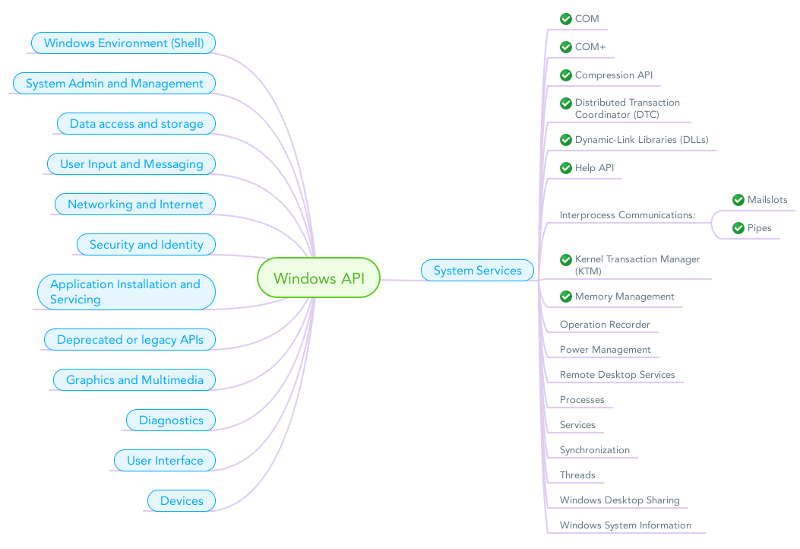
\includegraphics[scale=0.4]{res/MindMap2}
\caption{Рассматриваемые системные средства}
\end{figure}

\end{frame}

%------------------------------------------------
\section{COM/COM+}
%------------------------------------------------

\begin{frame}
\frametitle{COM/COM+}

\begin{block}{COM}
Component Object Model (объектная модель компонентов) - это технологический стандарт, предназначенный для создания программного обеспечения на основе взаимодействующих компонентов, каждый из которых может использоваться во многих программах одновременно.
\end{block}

\begin{block}{COM+}
Расширение стандартной COM модели, появившиеся в составе Windows 2000. Среди изменений можно отметить:
\begin{itemize}
\item автоматический пул потоков (создаваемый стандартным процессом-загрузчиком mtx.exe)
\item доступ к контексту, в котором выполняется компонент
\item интеграция с транзакциями монитора MS DTC (контекст COM+ может автоматически содержать в себе транзакцию MS DTC)
\end{itemize}
\end{block}

\end{frame}

%------------------------------------------------

\begin{frame}
\frametitle{COM/COM+ сравнение}

Одной из наиболее важных черт СОМ является ее способность предоставлять двоичный стандарт для программных компонентов.
\medskip

\begin{tabular}{|p{5.5cm}|p{5.5cm}|}
\hline 
C++-объект (экземпляр класса) & СОМ-объект \\ 
\hline 
Позволяет использовать только один общий интерфейс, представляющий собой множество С++ - методов & Обычно предоставляет более одного общего интерфейса \\ 
\hline 
Зависит от языка программирования & Обеспечивается независимость от языка - CОМ-объекты реализуются и используются в различных языках программирования \\ 
\hline 
Отсутствует встроенная возможность проверки версии & Поддерживается встроенный способ проверки версий объектов (независимо от положения в файловой системе) \\ 
\hline 
\end{tabular} 

\end{frame}

%------------------------------------------------

\begin{frame}
\frametitle{COM/COM+: список сущностей}

COM состоит из следующих сущностей:
\begin{itemize}
\item Константы
\item Нумераторы
\item Функции
\item Интерфейсы
\item Макросы
\item Записи реестра
\item Структуры
\end{itemize}

\end{frame}

%------------------------------------------------

\begin{frame}
\frametitle{COM/COM+: Константы}

\begin{itemize}
\item {Флаги доступа - ACTRL\_ACCESS\_ALLOWED и ACTRL\_ACCESS\_DENIED;}
\item {Флаги уровня аутентификации - определяют уровень аутентификации для обеспечения защиты и целостности данных;}
\item {Сервисные константы аутентификации - определяют службы проверки подлинности (NTLMSSP, Kerberos, Schannel);}
\item {Константы авторизации - определяют то, что авторизует сервер (к примеру, имя пользователя);}
\item {Коды ошибок - представляют список кодов ошибок, используемых API на базе COM, числовые значения кодов определены в файле Winerror.h;}
\item {Константы уровня представления - определяют уровень полномочий сервера, когда он выполняет роль клиента (анонимный, авторизированный, делегированный).}
\end{itemize}

\end{frame}

%------------------------------------------------

\begin{frame}[fragile]
\frametitle{COM/COM+: Нумераторы}


Их достаточно большое количество, но у них простая структура и понятные названия. Пример нумератор BINDSPEED, который показывает, как долго клиент будет ждать захвата объекта.

\begin{verbatim}
  typedef enum tagBINDSPEED { 
      BINDSPEED_INDEFINITE  = 1,
      BINDSPEED_MODERATE    = 2,
      BINDSPEED_IMMEDIATE   = 3
  } BINDSPEED;
\end{verbatim}

\end{frame}

%------------------------------------------------

\begin{frame}[fragile]
\frametitle{COM/COM+: Функции}

В распоряжении разработчика более 130 функций с диким количеством параметров! Запомнить их все крайне сложно.

\begin{verbatim}
  HRESULT CoGetInstanceFromFile(
      _In_opt_  COSERVERINFO *pServerInfo,
      _In_opt_  CLSID *pClsid,
      _In_opt_  IUnknown *punkOuter,
      _In_      DWORD dwClsCtx,
      _In_      DWORD grfMode,
      _In_      OLECHAR *pwszName,
      _In_      DWORD dwCount,
      _Inout_   MULTI_QI *pResults
);
\end{verbatim}

Они в основном управляет ресурсами, библиотеками, доступом и состоянием.

\end{frame}

%------------------------------------------------

\begin{frame}[fragile]
\frametitle{COM/COM+: Интерфейсы}

Больше 80 интерфейсов, обладающих различным набором функций.
\medskip

\begin{verbatim}
  typedef enum tagBINDSPEED { 
      BINDSPEED_INDEFINITE  = 1,
      BINDSPEED_MODERATE    = 2,
      BINDSPEED_IMMEDIATE   = 3
  } BINDSPEED;
\end{verbatim}

\end{frame}

%------------------------------------------------

\begin{frame}[fragile]
\frametitle{COM/COM+: Макросы}

Больше 80 интерфейсов, обладающих различным набором функций.
\medskip

Пример - два макроса, проверяющих существование описателя.
\begin{verbatim}
  #define FAILED(hr) (((HRESULT)(hr)) < 0)
\end{verbatim}

\begin{verbatim}
  #define SUCCEEDED(hr) (((HRESULT)(hr)) >= 0)
\end{verbatim}

\end{frame}

%------------------------------------------------

\begin{frame}[fragile]
\frametitle{COM/COM+: Записи реестра}

Аспектами функциональности COM управляют значения ключей в следующих ветках реестра:
\begin{itemize}
\item { \begin{verbatim}
HKEY_LOCAL_MACHINE\SOFTWARE\Classes
\end{verbatim} - Поддерживаемые форматы данных, информация о совместимости, программируемые идентификаторы и средства управления.}
\item { \begin{verbatim}
HKEY_LOCAL_MACHINE\SOFTWARE\Microsoft\Ole
\end{verbatim} - Параметры настройки права доступа и возможности безопасного вызова COM приложений.}
\item { \begin{verbatim}
HKEY_LOCAL_MACHINE\SOFTWARE\Microsoft\Windows NT\CurrentVersion
\end{verbatim} - Содержат информацию, связанную с функциональностью RPC COM.}
\end{itemize}

\end{frame}

%------------------------------------------------

\begin{frame}[fragile]
\frametitle{COM/COM+: Структуры}

Около 30 структур, связанных с авторизаций и аутентификацией.
\medskip

Пример - структура ACTRL\_ACCESS:

\begin{verbatim}
  typedef struct _ACTRL_ACCESS {
      ULONG                 cEntries;
      PACTRL_PROPERTY_ENTRY pPropertyAccessList;
  } ACTRL_ACCESS, *PACTRL_ACCESS;
\end{verbatim}

Первое поле указывает на количество, а второе на начало массива записей ACTRL\_PROPERTY\_ENTRY, каждая из которых содержит список записей, определяющих доступ к какому-либо объекту.

\end{frame}

%------------------------------------------------
\section{Compression API}
%------------------------------------------------

\begin{frame}
\frametitle{Compression API}

Сжатие позволяет выиграть пространство на диске за счёт тактов процессора, которые будут потрачены на декомпессию. Windows предоставляет следующие алгоритмы сжатия:

\begin{itemize}
\item XPRESS (COMPRESS\_ALGORITHM\_XPRESS) - очень быстрый и не требовательный к системным ресурсам
\item XPRESS с кодированием Хафмена (COMPRESS\_ALGORITHM\_XPRESS\_HUFF) - сжимает чуть лучше предыдущего
\item MSZIP (COMPRESS\_ALGORITHM\_MSZIP) - требует больше ресурсов, но обеспечивает хороший процент компрессии
\item LZMS (COMPRESS\_ALGORITHM\_LZMS) - алгоритм подходит для средних (от 2 МБ) и больших объёмов данных
\end{itemize}

\end{frame}

%------------------------------------------------

\begin{frame}[fragile]
\frametitle{Compression API: Процедура сжатия}

\begin{verbatim}
  CreateCompressor(// Создание компрессора
    // Алгоритм компрессии LZMS, блочный режим
    COMPRESS_ALGORITHM_LZMS|COMPRESS_RAW,
    // Опционально указывается алокатор памяти
    &AllocationRoutines,                    
    &Compressor); // Описатель компрессора

  Compress(       // Процедура сжатия блока.
    Compressor,   // Описатель компрессора
    InputData,    // Входной буфер, не сжатые данные
    BlockSize,    // размер не сжатого блока
    *OutputData,  // Буфер сжатия
    0,            // Размер буфера сжатия
    &CompressedBlockSize); // Размер сжатого блока
\end{verbatim}

При сжатии нужно перемещаться по входному (не сжатому) и выходному (сжатому) буферу, а после сохранить сжатый буфер.

\end{frame}

%------------------------------------------------

\begin{frame}[fragile]
\frametitle{Compression API: Процедура декомпрессии}

\begin{verbatim}
  CreateDecompressor( // Создание декомпрессора
    // Алгоритм компрессии LZMS, блочный режим
    COMPRESS_ALGORITHM_LZMS|COMPRESS_RAW,
    // Опционально указывается алокатор памяти
    &AllocationRoutines,                    
    &Compressor); // Описатель декомпрессора
   
  Decompress(     // Процедура сжатия блока.
    Decompressor, // Описатель декомпрессора
    InputData,    // Входные данные, сжатые
    CompressedBlockSize,   // Размер сжатого блока
    *OutputData,  // Выходные данные, не сжатые
    UncompressedBlockSize, // Размер не сжатого блока
    NULL);        // Количество разархивированных данных
\end{verbatim}

Как и раньше, нужно обеспечить смещение по каждому буферу и сохранить результат.

\end{frame}

%------------------------------------------------
\section{Distributed Transaction Coordinator (DTC)}
%------------------------------------------------

\begin{frame}
\frametitle{Distributed Transaction Coordinator (DTC)}

Координатор распределённых транзакций (DTC) - компонент Microsoft Windows, предназначенный для координации изменения данных на двух или более сетевых компьютерных системах.
\medskip

Координатор распределённых транзакций основан на технологии COM+ и включает в себя:
\begin{itemize}
\item менеджер транзакций;
\item журнал транзакций;
\item прокси (реализует интерфейсы DTC);
\item утилиты администрирования;
\item заголовочные файлы API.
\end{itemize}

\end{frame}

%------------------------------------------------

\begin{frame}[fragile]
\frametitle{Distributed Transaction Coordinator (DTC)}

При запросе фиксации или отката транзакции, менеджером транзакций выполняется двухфазный протокол фиксации. Во время первой фазы менеджеру ресурсов посылается запрос на подготовку к завершению, во время второй — на фиксацию или откат транзакции. По дереву, образованному вышестоящими и подчинёнными системами, рассылаются сообщения для подготовки к завершению, фиксации или отката. Любой узел дерева может прервать транзакцию до подтверждения подготовки к завершению.
\medskip

После того, как узел подтвердил подготовку, он остаётся в этом состоянии до фиксации или отката транзакции вышестоящим узлом. В случае сбоя и перезагрузки компьютера, менеджер транзакций запрашивает вышестоящий узел о дальнейшей судьбе подготовленных к завершению транзакций.

\end{frame}

%------------------------------------------------
\section{Dynamic-Link Libraries (DLLs)}
%------------------------------------------------

\begin{frame}
\frametitle{Dynamic-Link Libraries (DLLs)}

Ниже перечислены функции, которые используются в динамическом связывании:

\begin{itemize}
\item DisableThreadLibraryCalls - отключает уведомления DLL\_THREAD\_ATTACH и DLL\_THREAD\_DETACH для указанной динамически подключаемой библиотеки (DLL). 
\item DllMain - дополнительная точка входа в динамически подключаемую библиотеку (DLL).
\item FreeLibrary - уменьшает итоговое число ссылок на загруженные динамически подключаемые библиотеки (DLL). Когда итоговое число ссылок достигает нуля, модуль отменяет отображение в адресном пространстве вызывающего процесса.
\item FreeLibraryAndExitThread - уменьшает итоговое число ссылок загруженной динамически подключаемой библиотеки (DLL) до единицы, также, как это делает FreeLibrary , затем вызывает ExitThread, чтобы завершить работу вызывающего потока.
\end{itemize}

\end{frame}

%------------------------------------------------

\begin{frame}
\frametitle{Dynamic-Link Libraries (DLLs)}

Продолжение:
\begin{itemize}
\item GetDllDirectory - извлекает конкретную для приложения часть пути поиска, используемого, чтобы определить местонахождение DLLs для прикладной программы.
\item GetModuleFileName - извлекает полный путь доступа к файлу, содержащему указанный модуль, которым владеет текущий процесс.
\item GetModuleFileNameEx - извлекает полный путь доступа к файлу, содержащему заданный модуль.
\item GetModuleHandle - извлекает дескриптор указанного модуля, если файл был отображён в адресном пространстве вызывающего процесса.
\item GetModuleHandleEx - извлекает дескриптор указанного модуля, если файл был отображён в адресное пространство вызывающего процесса.
\end{itemize}

\end{frame}

%------------------------------------------------

\begin{frame}
\frametitle{Dynamic-Link Libraries (DLLs)}

Продолжение:
\begin{itemize}
\item GetProcAddress - извлекает адрес экспортируемой функции или переменной от заданной динамически подключаемой библиотеки (DLL).
\item LoadLibrary - отображает заданный исполняемый модуль в адресное пространство вызывающего процесса.
\item LoadLibraryEx - отображает указанный исполняемый модуль в адресное пространство вызывающего процесса. 
\item SetDllDirectory - добавляет каталог к пути поиска, используемый, чтобы определить местонахождение DLL для прикладной программы.
\end{itemize}

\end{frame}

%------------------------------------------------
\section{Help API}
%------------------------------------------------

\begin{frame}
\frametitle{Help API}

Справочное API позволяет открывать справочные каталоги, и получать оттуда материалы справки, такие как:
\begin{itemize}
\item Индексируемые справочные кончпекты (XHTML, HTML)
\item Не индексируемые изображения
\item Файлы CSS
\item Файлы JavaScript
\item Аудио/видео файл
\end{itemize}

\end{frame}

%------------------------------------------------

\begin{frame}
\frametitle{Help API}

Работа Help API осуществляется через ряд специфичных интерфейсов для объектов:
\begin{itemize}
\item ICatalog - интерфейс для объекта, хранящего состояние, т.е. хранящего описатель открытого каталога и всю информацию о нём
\item ICatalogRead - интерфейс для объекта, не хранящего своё состояние, т.е. обработка каталога осуществляется на основе полученных во время работы параметров
\item ICatalogReadWriteLock - интерфейс для объекта, блокирующего хранимый каталог, т.е. в процессе работы устанавливается замок на дескриптор каталога и всю информацию о нем
\item IHelpFilter -  коллекция критериев-фильтров, образованных парами ключ-значение
\item IHelpKeyValuePair - пара ключ-значение объектов IHelpFilter 
\end{itemize}

\end{frame}

%------------------------------------------------

\begin{frame}
\frametitle{Help API}

Продолжение:
\begin{itemize}
\item Ikeyword - интерфейс поиска по ключевым словам, содержит методы поиска информации по ключевым словам
\item IKeywordCollection – коллекция интерфейсов IKeyword 
\item ITopic - интерфейс тематического поиска, содержит методы поиска по заданной теме
\item ITopicCollection - коллекция интерфейсов Itopics
\item IndexException - интерфейс который получает свои характеристики от интерфейса IDispatch (общий интерфейс COM)
\end{itemize}

\end{frame}

%------------------------------------------------
\section{Interprocess Communications}
%------------------------------------------------

\begin{frame}
\frametitle{Interprocess Communications}

Операционная система Microsoft ® Windows ® предусматривает механизмы, которые облегчают обмен совместно использующейся информацией и данными между приложениями. В собирательном значении - это действия, включающие в работу механизмы, называемые межпроцессными взаимодействиями (interprocess communications) (IPC).
\medskip

Некоторые формы межпроцессного взаимодействия (IPC) облегчают разделение задания между несколькими специализированными процессами. Другие формы межпроцессорного взаимодействия (IPC) облегчают разделение задания между компьютерами в сети.

\end{frame}

%------------------------------------------------
\subsection{Mailslots}

\begin{frame}
\frametitle{Mailslots}

Почтовый слот в ядре Windows предоставляет разностороннюю связь. Любой процесс, который создает почтовый слот – это сервер почтового слота (mailslot server). Другие процессы, называемые клиентами почтового слота (mailslot clients), отправляют сообщения серверу почтового слота, записывая сообщение в его почтовом ящике.
\medskip

Входящие сообщения всегда добавляются в конец почтового слота. Почтовый слот в ядре Windows сохраняет сообщения до тех пор, пока сервер слота не прочтёт их. 
\end{frame}

%------------------------------------------------

\begin{frame}
\frametitle{Mailslots}

Клиент почтового слота может отправлять сообщение почтовому слоту на своем локальном компьютере, почтовому слоту на другом компьютере или всем почтовым слотам в ядре Windows с тем же самым именем на всех компьютерах в заданном сетевом домене. Сообщения, транслируемые всем почтовым слотам ядра Windows в домене, не могут быть длиннее, чем 400 байтов, принимая во внимание то, что сообщения, передаваемые в отдельно взятый почтовый слот, ограничиваются только максимальным размером сообщения, определяемым сервером почтового слота, когда он создавал этот слот в ядре Windows.

\end{frame}

%------------------------------------------------

\begin{frame}[fragile]
\frametitle{Mailslots}

\begin{verbatim}
  HANDLE CreateMailslot(    // Создание Mailslot
    LPCTSTR lpName,         // имя
    DWORD nMaxMessageSize,  // максимальный размер
    DWORD lReadTimeout,     // интервал тайм-аута чтения
    LPSECURITY_ATTRIBUTES lpSecurityAttributes //безопасность
  );

  BOOL GetMailslotInfo(       // Проверка данных
    HANDLE hMailslot,         // указатель на слот
    LPDWORD lpMaxMessageSize, // максимальный размер
    LPDWORD lpNextSize,       // размер следующего
    LPDWORD lpMessageCount,   // количество сообщений
    LPDWORD lpReadTimeout);   // тайм-аут.
\end{verbatim}

\end{frame}

%------------------------------------------------

\subsection{Pipes}
\begin{frame}
\frametitle{Pipes}

Имеются два типа каналов (абстрактных файлов) для двусторонней связи: анонимные (неименованные) и именованные каналы. Анонимные (или без имени) каналы (Anonymous pipes) дают возможность родственным процессам передавать информацию друг другу. Как правило, неименованный канал используется для переназначения стандартного ввода или вывода данных дочернего процесса так, чтобы он мог обмениваться данными со своим родительским процессом. Чтобы обмениваться данными в обоих направлениях (дуплексная работа), нужно создать два анонимных канала.
\medskip

Анонимные каналы не могут быть использованы в сети, и при этом они не могут быть использованы между несвязанными процессами.
\end{frame}

%------------------------------------------------

\begin{frame}
\frametitle{Pipes}

Именованные каналы (Named pipes) используются для передачи данных между процессами, которые являются не связанными процессами и между процессами на разных компьютерах. Как правило, процесс сервера именованного канала (named-pipe server) создаёт именованный канал с известным именем или именем, которое должно быть сообщено его клиентам.
\medskip

Процесс-клиент именованного канала (named-pipe client), который знает имя канала (абстрактного файла), может открыть его с другого конца, подчиняясь ограничениям доступа, которые определяются процессом сервера именованного канала. После этого, и сервер, и клиент присоединяются к каналу, они могут обмениваться данными, выполняя операции чтения и записи в канале.

\end{frame}

%------------------------------------------------

\begin{frame}[fragile]
\frametitle{Pipes}

\begin{verbatim}
  BOOL CreatePipe (   // Создание анонимного канала
    PHANDLE phRead,   // дескриптор файла для чтения
    PHANDLE phWrite,  // дескриптор файла для записи
    LPSECURITY_ATTRIBUTES lpsa,// безопасность
    DWORD nsize)      // опциональный размер канала

  BOOL WINAPI ReadFile(// Чтение из канала
    HANDLE hFile,      // файл, из которого читаем
    LPVOID lpBuffer,   // буфер-приемник данных
    DWORD nNumberOfBytesToRead, // размер буфера
    LPDWORD lpNumberOfBytesRead,// сколько прочитано
    LPOVERLAPPED lpOverlapped); // асинхронный обмен
\end{verbatim}

\end{frame}

%------------------------------------------------
\section{Kernel Transaction Manager (KTM)}
%------------------------------------------------

\begin{frame}
\frametitle{Kernel Transaction Manager (KTM)}
Транзакционная работа с файлами и реестром обеспечивается компонентом Kernel Transaction Manager. Не смотря на название, его можно использовать и из пользовательского режима. Более того, KTM поддерживает Microsoft Distributed Transaction Coordinator (MSDTC), таким образом, транзакции могут быть распределёнными двухфазными и затрагивать сразу несколько машин.
\medskip

Kernel Transaction Manager основывается на Common Log File System (CLFS) и не ограничивает использование транзакций конкретными типами ресурсов. Предоставляются стандартизированные реализации транзакционной работы с файловой системой и реестром. Вполне возможно добавить поддержку новых типов ресурсов самостоятельно. Таким образом, базовые функции KTM не специализированы, и их использование одинаково вне зависимости от типа ресурсов, над которыми производятся транзакции. Более того, в рамках одной транзакции допустимо обращаться к разным типам ресурсов.
\end{frame}

%------------------------------------------------

\begin{frame}
\frametitle{Kernel Transaction Manager (KTM)}
В рамках транзакции можно создавать и удалять файлы, менять их содержимое и атрибуты. Все эти изменения будут отменены в случае отката транзакции. Поддерживается также транзакционная работа с жёсткими и символическими ссылками.
\medskip

Следует отметить особую возможность — миниверсии. В рамках транзакции файл можно повторно открыть на чтение в состоянии до начала транзакции. Данная возможность позволяет выполнять сложные обновления файла на основе его текущего содержимого, без создания временных файлов или угрозы нарушения согласованности данных.
\end{frame}

%------------------------------------------------

\begin{frame}[fragile]
\begin{verbatim}
  HANDLE hTrans = CreateTransaction( // создание траназакции
       NULL,0, 0, 0, 0, NULL, _T("My NTFS Transaction"));

  USHORT view = 0xFFFE; // Открытие на запись (изменение)
  HANDLE hFile = CreateFileTransacted(
       _T("test.file"), GENERIC_WRITE, 0, NULL, CREATE_ALWAYS,
       0, NULL, hTrans, &view, NULL); // запуск транзакции

  DWORD dwWritten = 0; // Сколько реально данных записано
  string str = "Test String"; // данные файла
  WriteFile(hFile,str.c_str(),str.length(), &dwWritten, NULL);
  CloseHandle(hFile); // остановка транзакции

  CommitTransaction(hTrans);// или RollbackTransaction(hTrans);
  CloseHandle(hTrans);
\end{verbatim}
\end{frame}

%------------------------------------------------
\section{Memory Management }
%------------------------------------------------

\begin{frame}
\frametitle{Memory Management }

Управление динамической памятью в той или иной форме требуется в большинстве программ. Необходимость в этом возникает всякий раз, когда требуется создавать структуры данных, размер которых не может быть определен заранее на стадии создания программы. Типичными примерами динамических структур данных могут служить деревья поиска, таблицы имен и связанные списки.
\medskip

В Windows предусмотрены гибкие механизмы управления динамической памятью программы. На уровне WinAPI есть ряд функций, которые позволяют сообщать ядру о том, как нужно управлять памятью. Данные о том, какое количество памяти является реальным, а какое виртуальным может потребоваться системным твикерам или высокопроизводительным приложениям.

\end{frame}

%------------------------------------------------

\begin{frame}
\frametitle{Memory Management }

Список функций для управления памятью:
\begin{itemize}
\item AddSecureMemoryCacheCallback - регистрирует функцию обратного вызова, чтоб обратиться к ней, когда освободится надёжный объем памяти или изменятся параметры надёжности
\item CopyMemory - копирует блок памяти из одного места в другое
\item CreateMemoryResourceNotification – создаёт объект оповещения о ресурсах памяти
\item FillMemory – заполняет блок памяти присвоенным значением
\item GetLargePageMinimum – находит минимальный большой размер страницы (если процессор поддерживает большие страницы)
\end{itemize}

\end{frame}

%------------------------------------------------

\begin{frame}
\frametitle{Memory Management }

Продолжение:
\begin{itemize}
\item GetPhysicallyInstalledSystemMemory — находит объем оперативной памяти, установленной на компьютере
\item GetSystemFileCacheSize - находит текущие пределы размера для рабочих настроек системного кэша
\item GetWriteWatch - находит адреса страниц, к которым было произведено обращение на запись (в области виртуальной памяти)
\item GlobalMemoryStatusEx - обладает информацией о текущем использовании физической и виртуальной памяти
\item MoveMemory - перемещает блок памяти из одного места в другое
\item QueryMemoryResourceNotification - определяет состояние некого объекта в памяти
\end{itemize}

\end{frame}

%------------------------------------------------

\begin{frame}
\frametitle{Memory Management }

Продолжение:
\begin{itemize}
\item RemoveSecureMemoryCacheCallback — отменяет регистрацию функции обратного вызова, ранее зарегистрированную с помощью функции AddSecureMemoryCacheCallback
\item ResetWriteWatch — отключает отслеживание состояния раздела виртуальной памяти
\item SecureMemoryCacheCallback — функция приложения, которая вызывается, когда освобождается надёжный объем памяти или изменятся параметры надёжности
\item SecureZeroMemory — заполняет блок памяти нолями
\item SetSystemFileCacheSize — ограничивает размер рабочих настроек для кэша файловой системы
\item ZeroMemory - заполняет блок памяти нолями
\end{itemize}

\end{frame}

%------------------------------------------------
\section{Заключение}
%------------------------------------------------

\begin{frame}
\frametitle{Заключение}

Далее следует рассматривать следующие разделы MSDN:

\begin{itemize}
\item Operation Recorder (Контроллер записи)
\item Power Management (Управление энергопотреблением)
\item Remote Desktop Services (удалённый рабочий стол)
\item Processes (Процессы)
\item Services (Службы)
\item Synchronization (Синхронизация)
\item Threads (Потоки)
\item Windows Desktop Sharing (совместное использование рабочего стола)
\item Windows System Information (Информация о системе)
\begin{itemize}
    \item Handle and Objects (Описатели и объекты):
    \item Registry (Реестр)
    \item Time (Время)
    \item Time Provider (Служба времени)
\end{itemize}
\end{itemize}
\end{frame}
%------------------------------------------------
\section{Ссылки}
%------------------------------------------------

\begin{frame}
\frametitle{Ссылки}

\begin{itemize}
\item COM - \url{https://msdn.microsoft.com/ms693341}
\item COM+ - \url{https://msdn.microsoft.com/ms687816}
\item Compression API - \url{https://msdn.microsoft.com/hh437596}
\item Distributed Transaction Coordinator (DTC) - \url{https://msdn.microsoft.com/ms686108}
\item Dynamic-Link Libraries (DLLs) - \url{https://msdn.microsoft.com/ms682599}
\item Help API - \url{https://msdn.microsoft.com/hh447319}
\item Interprocess Communications: - \url{https://msdn.microsoft.com/aa365574}
    \begin{itemize}
    \item Mailslots - \url{https://msdn.microsoft.com/aa365580}
    \item Pipes - \url{https://msdn.microsoft.com/aa365781}
    \end{itemize}
\item Kernel Transaction Manager (KTM) - \url{https://msdn.microsoft.com/aa366288}
\item Memory Management - \url{https://msdn.microsoft.com/aa366782}
\end{itemize}

\end{frame}

%------------------------------------------------
\section{Вопросы}
%------------------------------------------------

\begin{frame}
\Huge{\centerline{Вопросы?}}
\end{frame}

%----------------------------------------------------------------------------------------

\end{document} 
